This chapter covers details of camera, the main sensor used in \acrshort{vo}. Different types of cameras, advantages and drawbacks with important properties for \acrshort{vo} implementation, selection of camera and calibration are explained. 

\section{Classification of Camera}
Cameras can be classified mainly into two types :
\begin{enumerate}
	\item Passive Camera
	\begin{enumerate}
		\item Monocular
		\item Stereo
		\item Omnidirectional
	\end{enumerate}
	\item Active Camera
	\begin{enumerate}
		\item Time of flight(TOF)
		\item RGB-Depth
	\end{enumerate}
\end{enumerate}
Passive cameras are mostly used in \acrshort{vo} implementation. Some common types are shown in the figure \ref{fig:cameras}.
\begin{figure}[h]
	\centering
	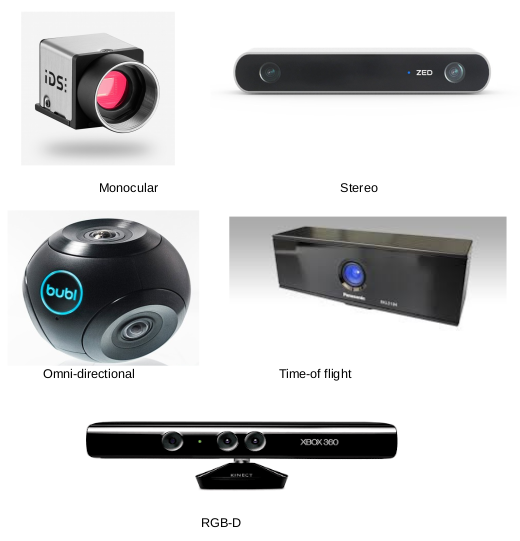
\includegraphics[width=0.9\textwidth]{cameras}
	\caption{Different types of cameras used in \acrshort{vo} source:\cite{ids},\cite{kinect},\cite{zed}, \cite{omni},\cite{tof}}
	\label{fig:cameras}
\end{figure}


\section{Important Properties}
There are some criteria to select the proper camera model in order to achieve high accuracy and robustness. First important property is shutter technology. The rolling shutter cameras may consist geometric distortions in the image for moving camera or dynamic scene condition which reduces the accuracy especially direct \acrshort{vo} methods (section \ref{direct}) as they don't optimize geometric noise. Another important factor is Field of view (FOV) of a camera. Large \acrshort{fov} cameras would have enough information (features) to track the motion which increases robustness to large rotation. Higher camera resolution can increase the accuracy of 3D pose estimation of the features but at the same time it will increase the computation cost due to more number of pixels in one image. Auto-exposure may reduce the accuracy of direct \acrshort{vo}. Therefore, It is important to use fixed-focus camera for the direct approaches. Finally the suitable size of lens object can reduce the effect of vignetting(a radial falloff of intensity from the image center) \cite{vignette} which occurs due to blockage of light due to some camera parts or hoods attached to lens.

\section{Camera Selection}
Monocular cameras are consist of one image sensor and lens. Depending on types of lens they can be modeled as pinhole, fisheye(wide \acrshort{fov}) or omnidirectional\cite{multiview_geometry}. The main disadvantage of monocular camera is that they can not estimate the true depth of the scene. Absolute scale can be estimated with using some prior knowledge like known object-size \cite{citymodel}, deep learning methods as explained in \cite{synthetic}, \cite{deepl}  or geometric constraints like known camera heights for planer motion as described in \cite{ground}, \cite{geometric} and \cite{planer} or fusion with some extra sensor like \acrshort{imu}, \acrshort{gps} or 2D \acrshort{lidar} etc. \\
\newline
Stereo cameras are consist two image sensors inspired from humans with fixed distance(baseline) between them. Both cameras are synchronized to capture images at the same time. Stereo camera can sense the depth of the world by finding correspondences in the left and right image taken at same time. The accuracy of depth estimation depends on the baseline. When depth increases with fixed baseline, it can be gradually degraded to monocular case. Stereo camera required good calibration, stereo rectification, undistortion. \\
\newline
A combination of both the types discussed above is call as RGB-D camera. It consists of a depth sensor in addition to monocular sensor based on time of flight. For every pixel the depth can be measured and register into depth map for every image with no need of stereo. Limitation of RGB-D is that they can be either used for indoor application or upto some limit of depth. The table \ref{table:cameracomp} shows some of the advantages and disadvantages of these cameras.\\
\begin{table}[h!]
	\centering
	\begin{tabular}{ |m{0.12\linewidth} | m{0.40\linewidth} | m{0.40\linewidth} |}
		\hline 
		\textbf{Camera} & \textbf{Advantages}  & \textbf{Disadvantages} \\ [1ex] \hline
		Monocular & \begin{itemize} 
				 		\item Cheaper, light weight
						\item Small size, low computational cost 
						\item Simple calibration 
				   \end{itemize} & 
			       \begin{itemize} 
			       	\item Suffers from scale ambiguity
			       	\item \acrshort{vo} fails in pure rotations
			       	\item Slow \acrshort{vo} initialization
			       \end{itemize} \\ \hline
		Stereo & \begin{itemize} 
					\item 3D vision from one stereo pair
					\item Easy \acrshort{vo} initialization
				\end{itemize} & 
				\begin{itemize} 
					\item Expensive and complex calibration
					\item High processing time and cost
					\item Complex synchronization
				\end{itemize} \\ \hline
		RGB-D  & \begin{itemize} 
					\item Provides depth map 
					\item Easy \acrshort{vo} initialization
				\end{itemize} & 
				\begin{itemize} 
					\item Limited to indoor and small depth environment
					\item High power consumption
					\item Complex calibration
				\end{itemize} \\ \hline
	\end{tabular}
	\caption{Advantages and disadvantages of cameras used in \acrshort{vo}}
	\label{table:cameracomp}  
\end{table}
\newline
Based on discussion of camera properties above monocular cameras were selected due to their advantages. The two different type of monocular cameras were selected based on availability namely SICK-Picocam (model-I2D304C-RCA11) and a rolling shutter Genius widecam (F100) in order to compare the different technology. Best performing camera will be selected for the adaptation and further research. Table \ref{table:camera_prop} illustrate the properties of these cameras in comparison with IDS UI-3241LE which is used in TUM- benchmark dataset \cite{engel2016photometrically}.
\begin{table}[h!]
	\centering
	\begin{tabular}{ | l | l | l | l |}
		\hline
		\textbf{Model} & \textbf{SICK Picocam}  & \textbf{Genius widecam}  & \textbf{IDS UI-3241LE}  \\  
		              & \textbf{I2D304C-RCA11} & \textbf{F100} &  \\  
		\hline
		Shutter technology & Global & Rolling shutter & Global and Rolling \\ 
		\hline
		Lens type         & C-mount & attached        & S-mount \\ 
		\hline
		FPS               & 19      & 30              & 60\\ 
		\hline
		Resolution       & 2048*2048  &  1280 * 720   & 1280 *1024 \\
		 \hline
		Exposure time (ms) & 0.0009 - 2000 & auto &    \\
		 \hline
		Sensor size (mm) & 11.26 x 11.26 & 6.784 x 5.427 &  \\
		 \hline
		FOV (degree) &  90(diag) &  120 & 98 x 79  \\
		 \hline
		Lens &  Kowa   &   & Lensagon \\
		     &  LM8HC  &   & BM4018S118  \\
		 \hline
	\end{tabular}
    \caption{Comparison of properties of cameras used in this thesis with IDS UI-324LE used in TUM-benchmark dataset}
    \label{table:camera_prop}
\end{table}
\section{Camera Calibration}

For any \acrshort{vo} method camera calibration is an important part. Though some cameras are manufactured very well, they still have some distortions. Using cameras directly without calibration may lead to wrong trajectory estimation and \acrshort{vo} may not work well. Camera calibration can be classified into two types 1. Geometric and 2. Photometric. Geometric calibration covers intrinsic and distortion parameters. While photometric focuses on the effect of shutter speed, motion blur and vignette. It is mostly recommended for cameras which have rolling shutter and auto-exposure technology. Moreover, It is also recommended for direct approaches which use monitors image pixel intensity values for tracking \cite{yang2018challenges}. This section will discuss only geometric calibration. Photometric calibration is not in the scope of this thesis because photometric type is complex procedure and not compulsory for any \acrshort{vo} approaches. The more details about photometric calibration and its effects can be found in \cite{yang2018challenges} ,\cite{photometrically}, \cite{bergmann2017online} and \cite{vignette}.\\

\subsection{Pinhole Camera Model}
Monocular camera with normal lens can be simply model as pinhole camera model as shown in figure \ref{fig:pinhole}. A 2D image point  $ m = [u,v]^{T} $ on image with corresponding 3D point $ M = [ X,Y Z]^{T} $ in world can be formed by an optical ray from M passing through camera optical center C by intersecting image plane at m. The relation between M and m in homogeneous coordinates can be given by: 
\begin{equation*}
sm= KTM 
\end{equation*} 
\begin{equation*}
K = \begin{bmatrix}
f_{x} & \gamma & u_{o} \\
0    &  f_{y} & v_{o} \\
0    &   0    & 1 \\
\end{bmatrix}
\end{equation*} 
and matrix $ T = R t $
\begin{equation*}
P = \begin{bmatrix}
r_{11} & r_{12} & r_{13} & t_{1} \\
r_{21} & r_{22} & r_{23} & t_{2} \\
r_{31} & r_{32} & r_{33} & t_{3} \\
\end{bmatrix}
\end{equation*} 
where s is scale factor. Camera matrix K is known as camera intrinsic matrix with $ (u_{0},v_{0}) $ being a principal point,$ (f_{x},f_{y}) $ being the focal length in pixels in x and y direction, and $ \gamma $ is the skew between both image axis. T is the 3x4 transformation matrix with R and t being rotation and translation from world to camera frame also known as extrinsic parameters.\\
\begin{figure}[h!]
	\centering
	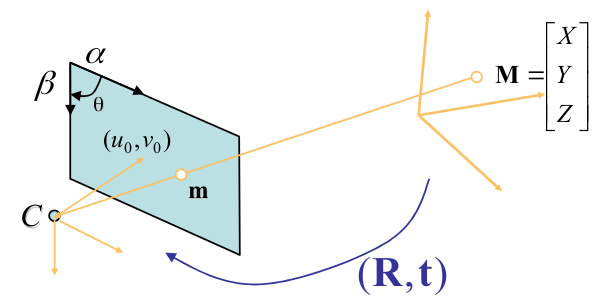
\includegraphics[width=0.8\textwidth]{pinhole}
	\caption{Pinhole camera model. C is camera center, m is 2D image point corresponding to 3D object point M, R and t are rotation and translation resp. source:\cite{cameracalib}}
	\label{fig:pinhole}
\end{figure}
\newline
The purpose of camera calibration is to compute these parameters known as intrinsic and extrinsic parameters. The combination of K and T is also known as projection matrix denoted by $ P = K \begin{bmatrix} 
            R & t \\
            \end{bmatrix} $.
The are total 11 parameters to be determine where total degrees of freedom are 6 and 5 intrinsic parameters $ (f_{x},f_{y},u_{0},v_{0}, \gamma) $. There exists many techniques of geometric calibration based on type of the reference objects. They can be found in \cite{cameracalib}. In this thesis 2D plane based technique \cite{zhangcalib} ,\cite{sturmcalib} is used due to its simplicity and sufficient accuracy. The mathematical derivation can be found in \cite{cameracalib}.\\
\newline
Camera lens may also consists distortion. There are two types of distortion can be found in pinhole camera lens: radial and tangential distortion. Radial distortion shown in figure \ref{fig:distortion} generates due to distortion of optical rays at the lens edge which depends on the size of lens. i.e. smaller lens consist higher radial distortion. The relation between distorted and undistorted pixels coordinates can be estimated as:
\begin{equation*}
p_{undistorted} = p_{distorted} /(1+ k_{1}r^{2}+k_{2}r^{4}+k_{3}r^{6})
\end{equation*} 
where $ k_{1},k_{2},k_{3} $ are known as radial distortion coefficients.\\
\newline
Tangential distortion generally occurs due to not parallel lens and sensor. It depends on mounting and manufacturing of camera. There are only two coefficients which needs to corrected known as $p_{1} and p_{2} $. So in normal camera calibration there are five distortion parameters and 11 intrinsic parameters needs to be estimated. There are some open-source software tools are already available with code. such as Matlab, OpenCV etc. OpenCV camera calibration module has been used in this scope. 
\begin{figure}[h!]
	\centering
	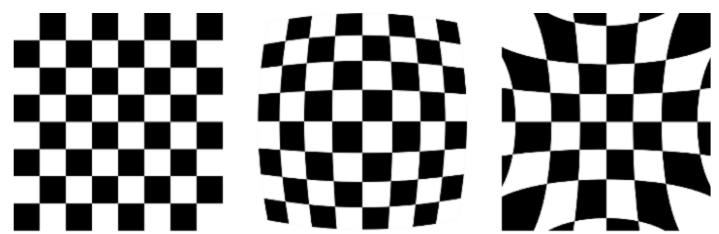
\includegraphics[width=0.8\textwidth]{distortion}
	\caption{Radial distortion created by camera lens source : \cite{opencvcalib}}
	\label{fig:distortion}
\end{figure}

\subsection{Calibration Procedure}
This section covers the calibration procedure in brief. Different types of calibration pattern can be used such as chessboard, AR tags, symmetric and asymmetric circular grid as shown in figure \ref{fig:pattern}. In this thesis work a symmetric circular grid pattern is used for picocam and chessboard pattern is used for genius widecam. The size of circular pattern is relatively larger than that of chessboard because picocam has higher image resolution.\\
\begin{figure}[h!]
	\centering
	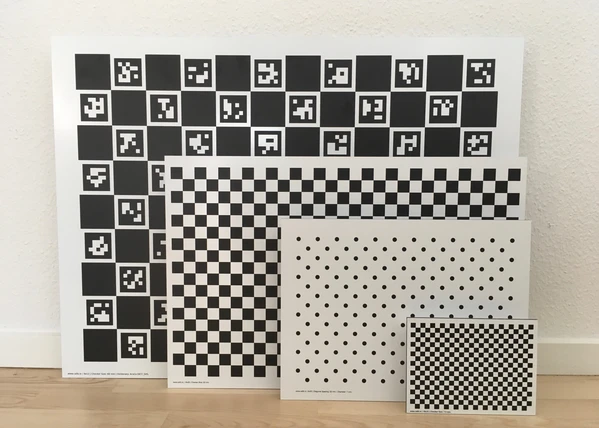
\includegraphics[width=0.8\textwidth]{pattern}
	\caption{Types of calibration pattern used for camera calibration. such as AR tags, chessboard, circles grid. source:\cite{calibio}}
	\label{fig:pattern}
\end{figure}
\newline
The general steps are as follows \cite{cameracalib}:
\begin{enumerate}
	\item Print the target pattern with sufficient size and fix it to planer surface.
	\item Grab some images of the pattern in different orientation and positions by moving either the target or camera.
	\item Detect the all corners or features of the pattern in all images.
	\item Compute the intrinsic and extrinsic parameters.
	\item Estimate the distortion coefficient.
	\item Refine all parameters and project the 3D object points using computed parameters.
	\item Compute the reprojection error, accept the result if error is with in limit otherwise repeat the procedure by taking more number of images until error is in limit.
\end{enumerate}

\subsection{Recommendations for good calibration}
Accurate intrinsic camera calibration is one of the most important factor for \acrshort{vo} algorithms regardless of its approach. This section describes some of the best practices to achieve higher accuracy. They are:
\begin{enumerate}
	\item The target pattern should be right size. Optimal should be nearly half of the total area seen in front of camera. Calibration accuracy also depends on target print quality.
	\item Camera and lens should be focused on the same distance where target is. It should remains unchanged during the \acrshort{vo} run. 
	\item Images should be collected from different areas and in all orientations. It is recommended to estimate the lens distortion and camera focal length.
	\item The surrounding area should have proper and rather diffused lighting. 
	\item The number of images should be enough covering all parts of areas.
	\item Either target or camera should be mount rigidly during the whole process. Camera should not move during image capturing.
	\item If there is any bad images which consist higher reprojection error then it should be remove.
	\item Lower reprojection error doesn't mean that the camera calibration is accurate. It can also be case of overfitting. Ever reprojection error should be analyse and images with higher error should be removed and recalibration should be done until satisfactory results has arrived.
\end{enumerate}

\subsection{Calibration result}
As discussed two cameras have been selected in this scope of work. Both cameras were calibrated using different target patterns. Picocam has been calibrated using symmetric circular grid as shown in figure \ref{fig:circular_grid}. while Genius widecam (webcam) has been calibrated with help of 8 x 8 size as shown in figure \ref{fig:chessboard}. More than 150 images were taken for both cameras. The resolution for Picocam is 1024 x 1024 and for webcam it is 1080 x 720 pixels. The calibration result for both cameras is attached can be found in \ref{section:A.2}. The figure \ref{fig:pattern_view} shows camera poses taken in all possible locations with respect to the pattern. The average reprojection error estimated for picocam below 0.010 pixels which can be seen in figure \ref{fig:reproj}.
\begin{figure}[h]
	\centering
	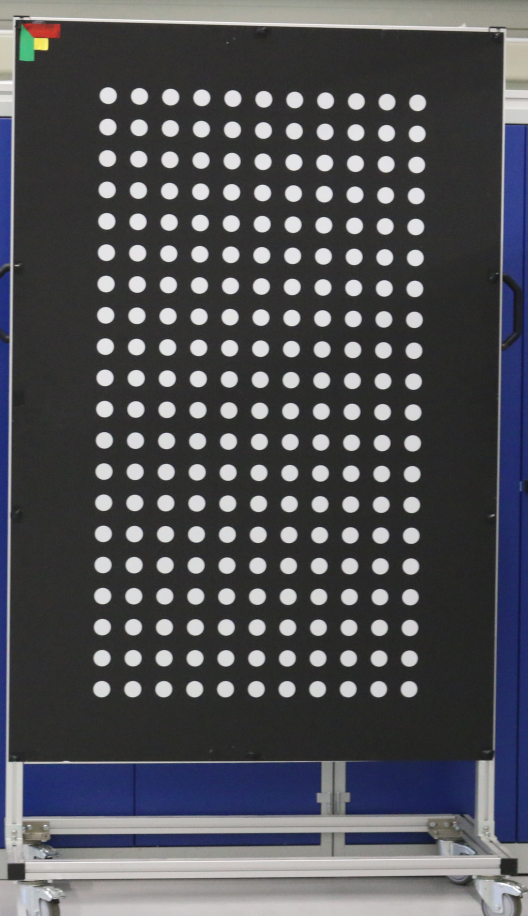
\includegraphics[width=0.4\textwidth]{circular_grid}
	\caption{Symmetric circular pattern used for Picocam Calibration.}
	\label{fig:circular_grid}
\end{figure}
\begin{figure}[h]
	\centering
	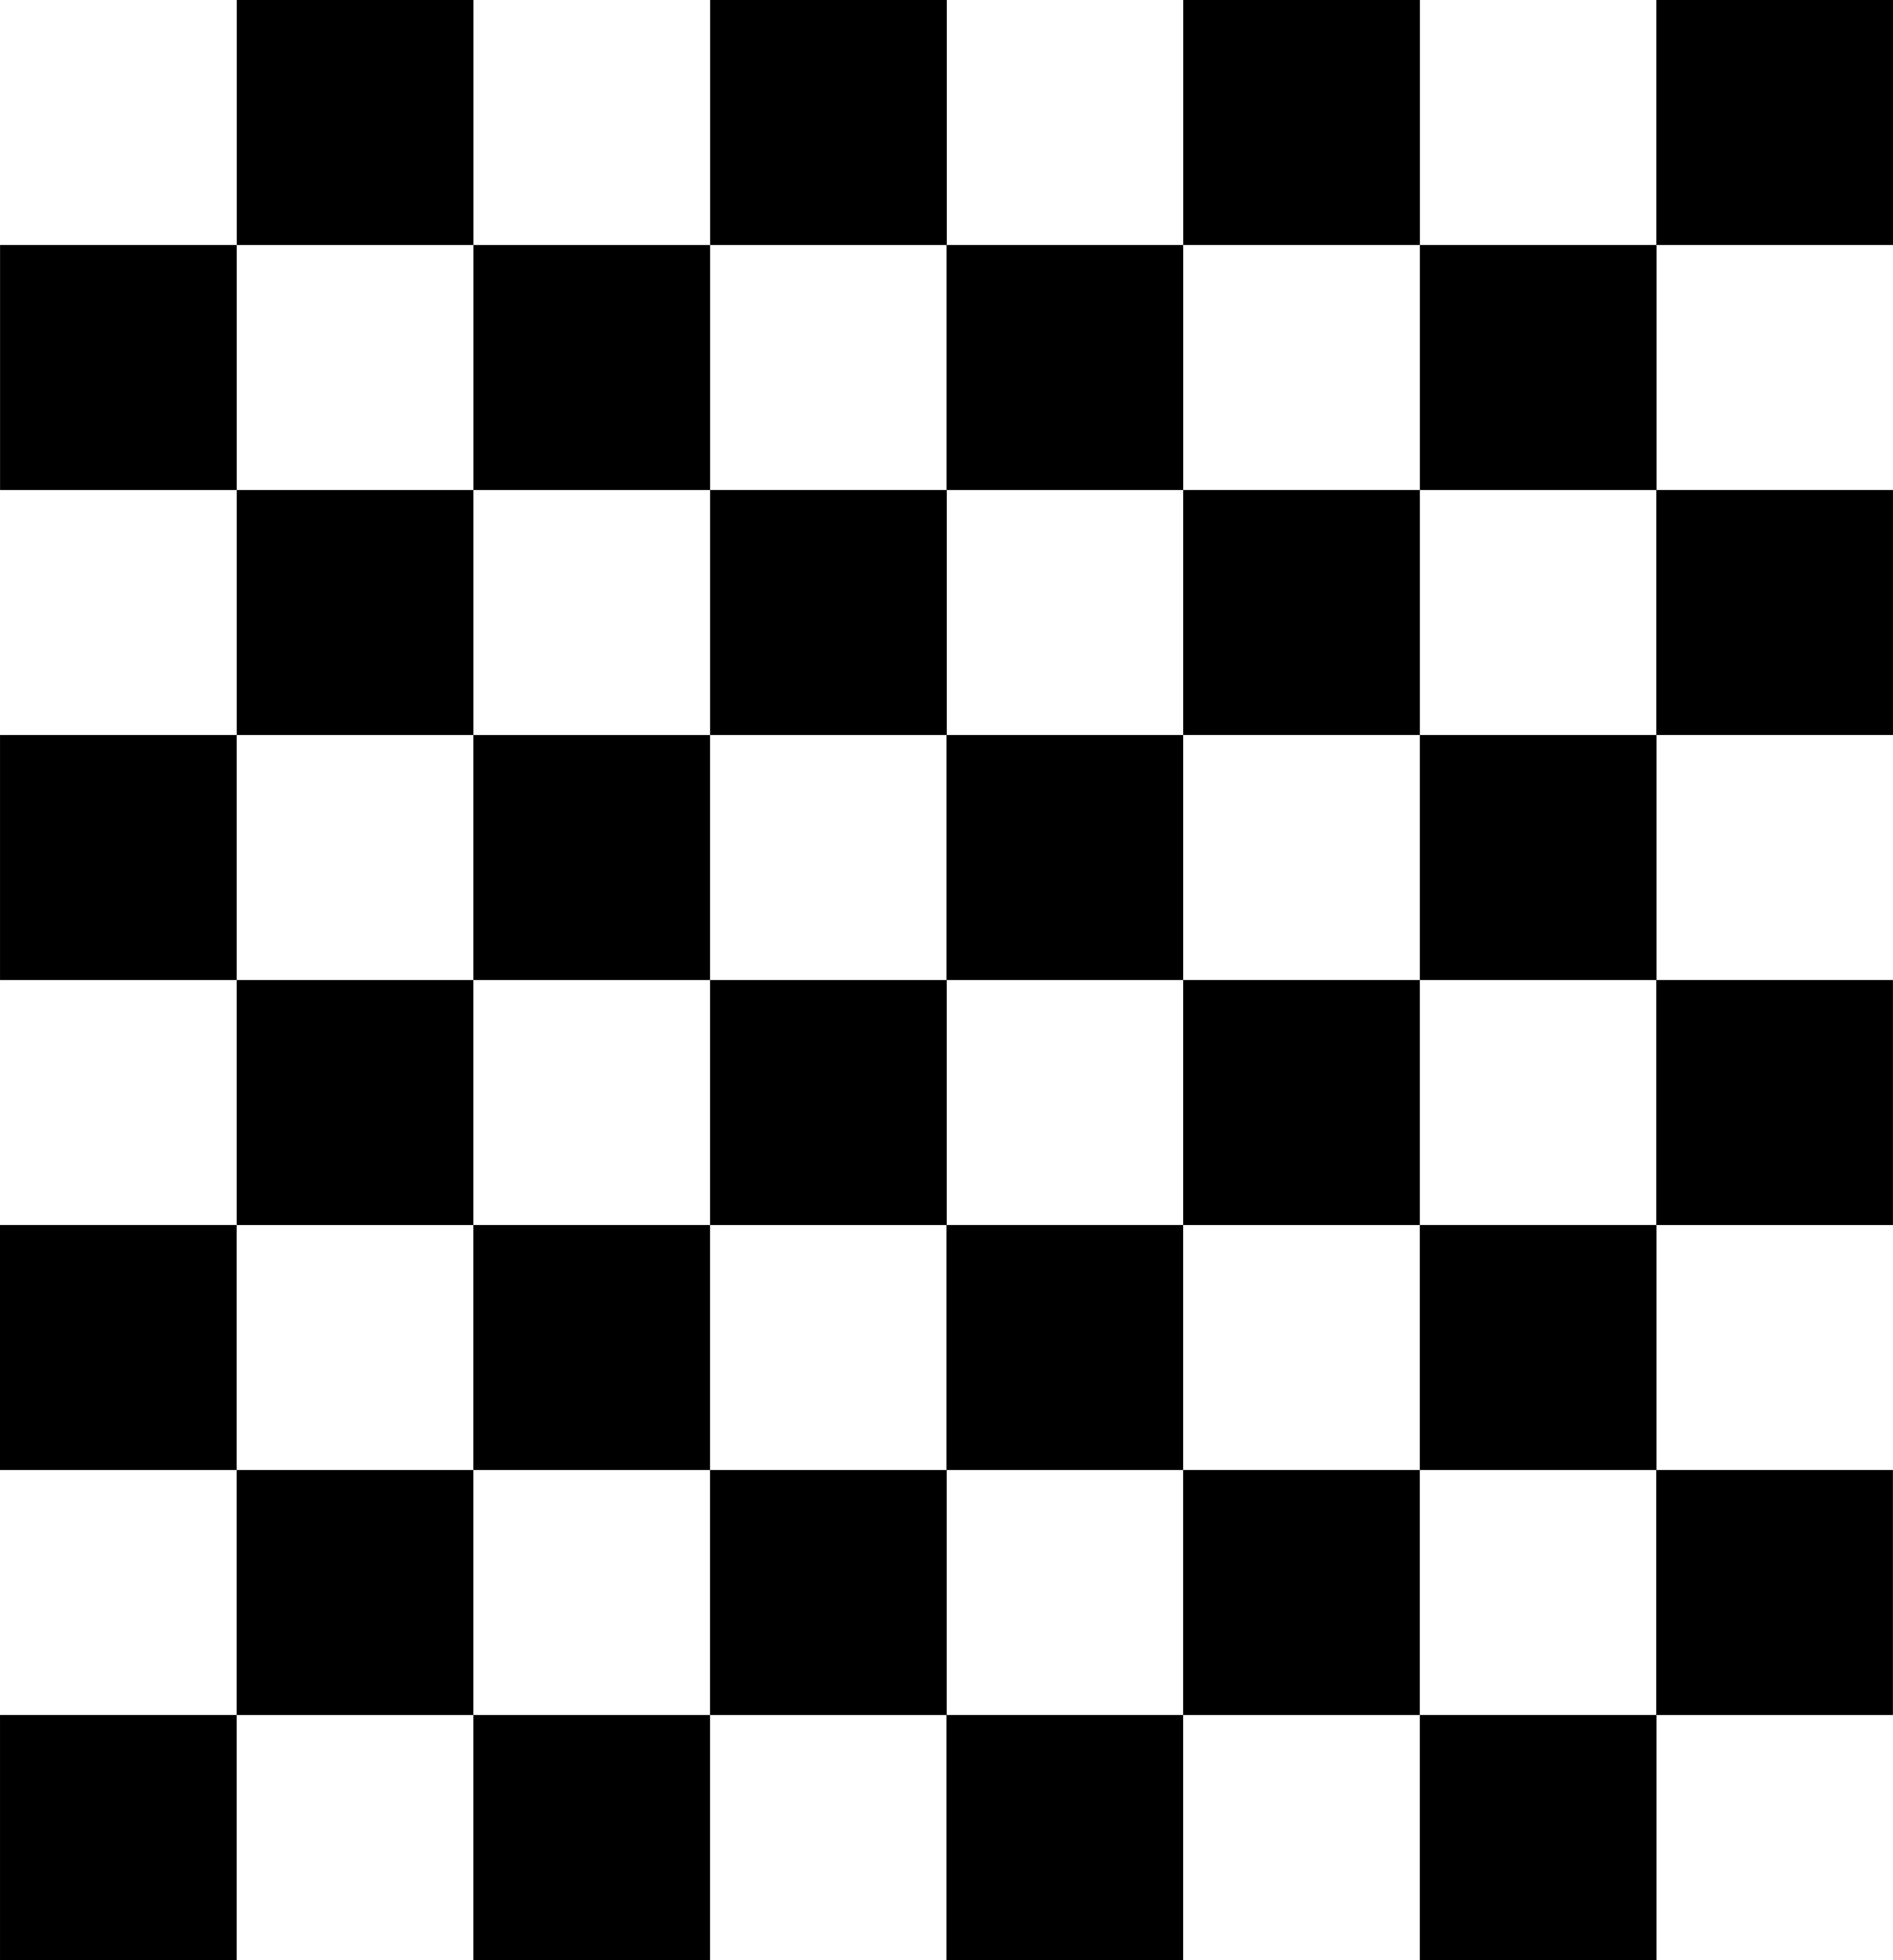
\includegraphics[width=0.5\textwidth]{chessboard}
	\caption{Chessboard pattern of size 8 x8 used for Genius widecam calibration.}
	\label{fig:chessboard}
\end{figure}
\begin{figure}[h!]
	\centering
	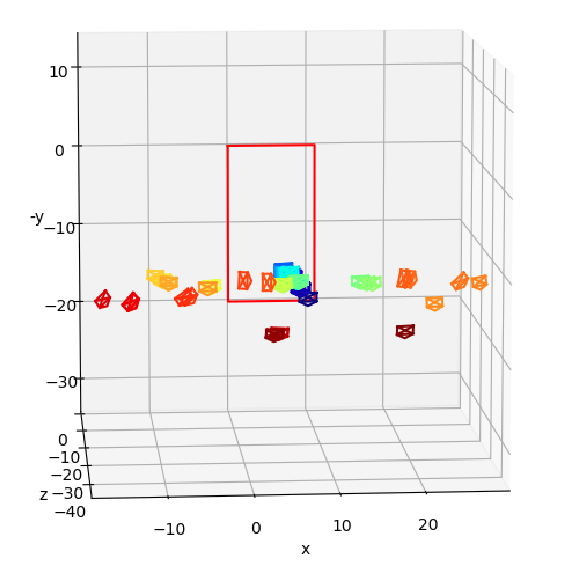
\includegraphics[width=0.8\textwidth]{pattern_view}
	\caption{Pattern centric view with rectangle as pattern and pentagons as camera}
	\label{fig:pattern_view}
\end{figure}
\begin{figure}[h!]
	\centering
	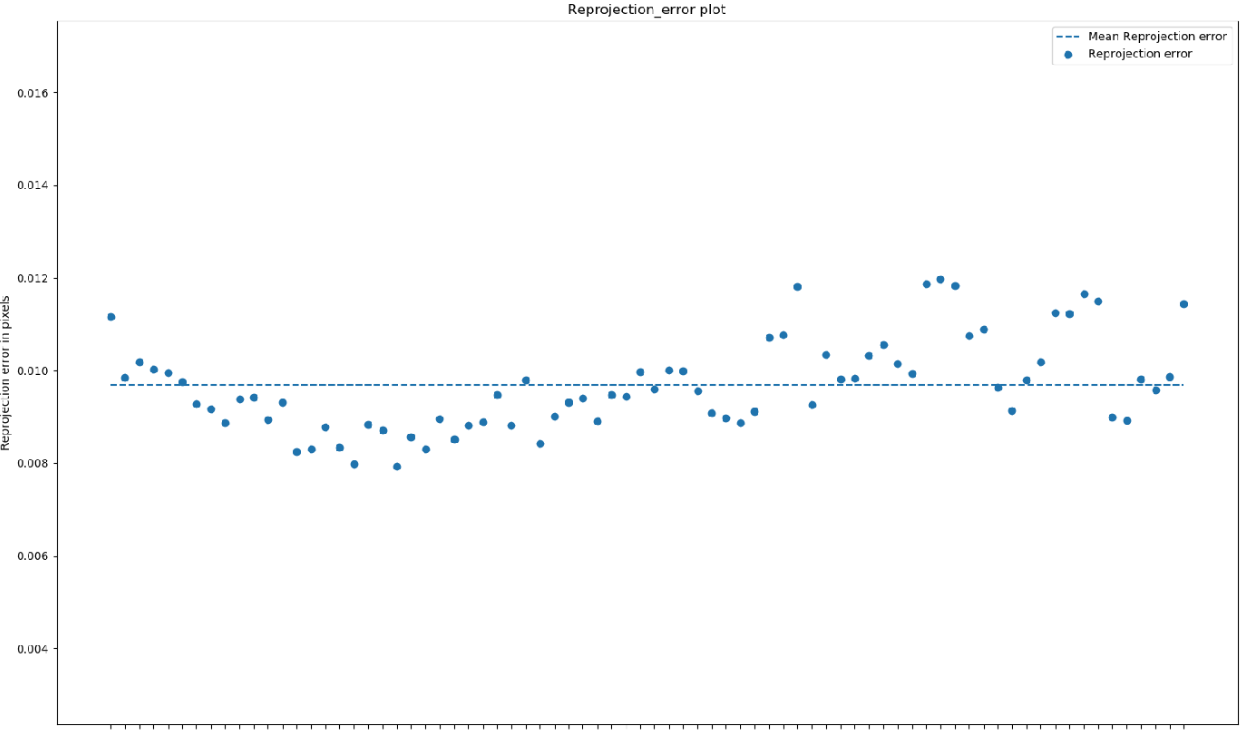
\includegraphics[width=1.0\textwidth]{reproj_error}
	\caption{Reprojection error plot for picocam}
	\label{fig:reproj}
\end{figure}
